The tau identification strategy described previously can be extended by
looking at the different hadronic decay modes of the tau individually.
The dominant hadronic decays of taus consist of a one or three charged
$\pi^{\pm}$ mesons and up to two $\pi^0$ mesons and are enumerated in ``Hadronic
decay mode'' section of 
table~\ref{tab:decay_modes}.  The majority of these decays proceed through
intermediate resonances and each of these decay modes maps directly to a tau
final state multiplicity. Each intermediate resonance has a different invariant
mass (see figure~\ref{fig:trueInvMass}).  This implies that the problem of
hadronic tau identification can be re-framed from a global search for
collimated hadrons satisfying the tau mass constraint into a ensemble of
searches for single production of the different hadronic tau decay resonances.
The Tau Neural Classifier algorithm implements this approach using two
complimentary techniques: a method to reconstruct the decay mode and an
ensemble of neural network classifiers used to identify each decay mode
resonance and reject quark and gluon jets with the same final state topology.

\begin{table}
   \centering
   \begin{tabular}{l c r r }
      Visible Decay Products  & Resonance & Mass (\MeVcc) & Fraction~\cite{PDG} \\
      \hline
      $\pi^{-}$                    & -      & 135  & 10.9\% \\
      $\pi^{-}\pi^0$               & $\rho$ & 770  & 25.5\% \\
      $\pi^{-}\pi^0\pi^0$          & $a1$   & 1200 & 9.3\% \\
      $\pi^{-}\pi^{-}\pi^{+}$      & $a1$   & 1200 & 9.03\% \\
      $\pi^{-}\pi^{-}\pi^{+}\pi^0$ & $a1$   & 1200 & 4.5\% \\
      \hline
      Total & & & 59.2\% \\
      \hline
      Other hadronic modes & & & 5.59\% \\
   \end{tabular}
   \label{tab:decay_modes}
   \caption{Resonances and branching ratios of the dominant hadronic decays of
   the tau lepton.  The decay products listed correspond to a negatively
   charged tau lepton; the table is identical under charge conjugation.}
\end{table}

\begin{figure}[thbp]
   \begin{center}
      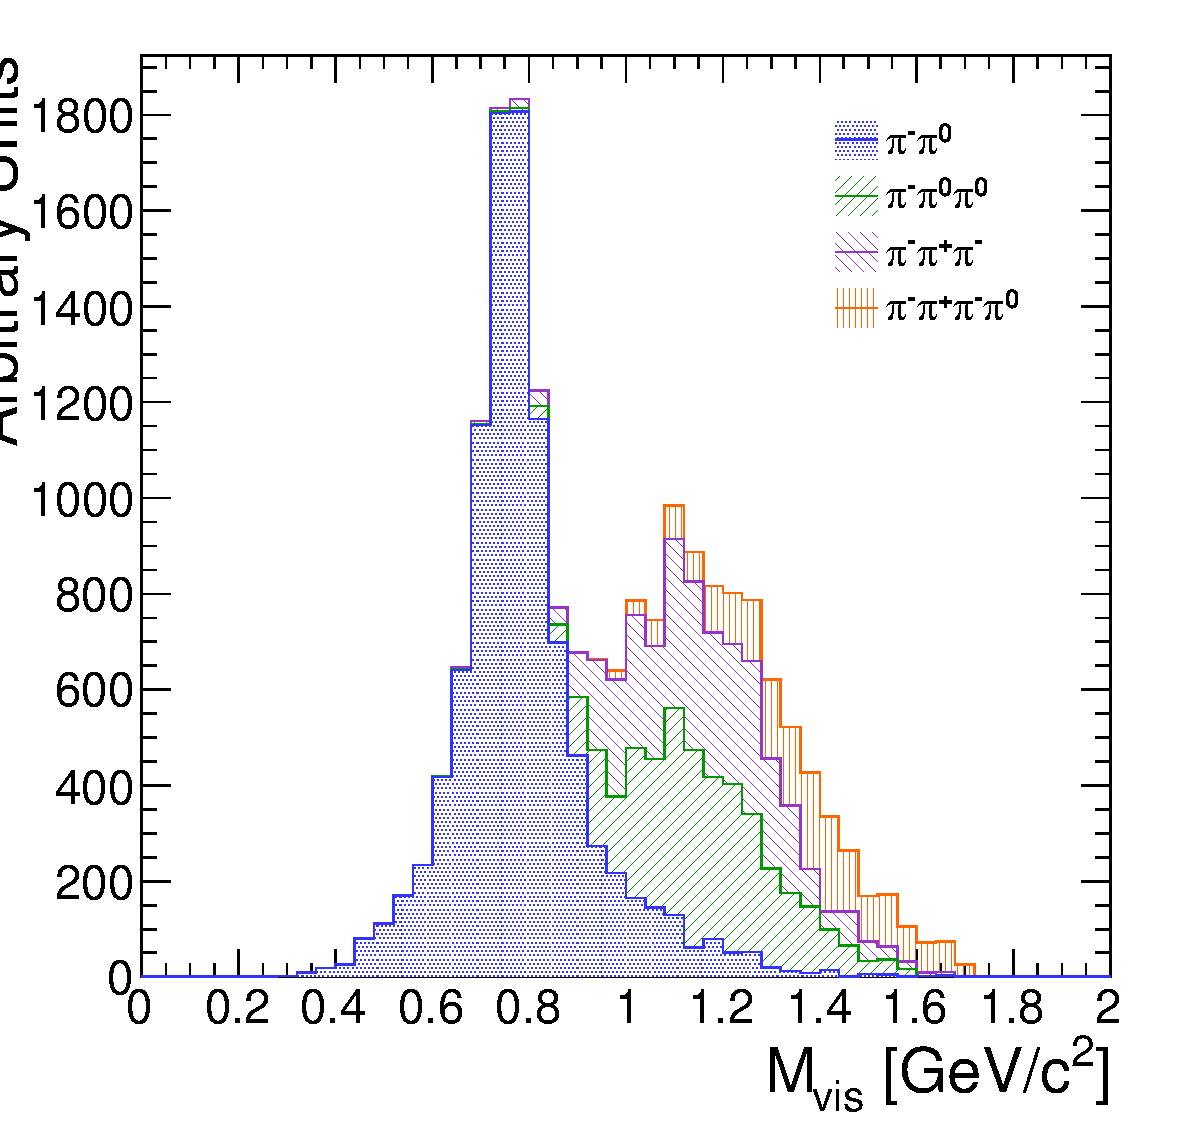
\includegraphics[width=90mm]{figures/truthIMvsDM.pdf}
   \end{center}
   \caption{The invariant mass of the visible decay products in hadronic tau
   decays.  The decay mode $\tau^{-} \rightarrow \pi^{-} \nu_\tau$ is omitted.
   The different decay modes have different invariant masses corresponding to
   the intermediate resonance in the decay.}
   \label{fig:trueInvMass}
\end{figure}
